\documentclass[
	classe=$2^{de}$
]{exercice}

\title{Activité : tirage de cartes}

\begin{document}

\maketitle

On considère un jeu de cartes de 40 cartes :
\begin{itemize}
	\item Quatres couleurs : cœur, pique, trèfle et carreau.
	\item $10$ cartes par couleur, numérotées de $1$ à $10$.
\end{itemize}

\begin{enumerate}
	\item Donner la probabilité des évènements suivants :
	      \begin{itemize}
		      \item «La carte tirée est un cœur» : \correctionDots{$1/4$}
		      \item «Le numéro de la carte tirée est 4» : \correctionDots{$1/10$}
		      \item «Le numéro de la carte tirée est inférieur ou égal à 6» : \correctionDots{$6/10$}
	      \end{itemize}
	\item On considère maintenant qu'on tire une \textit{première carte}, on la remet dans le jeu, puis on tire une \textit{deuxième carte}.

	      À chaque tirage, on regarde si la carte est un cœur, un pique, ou autre.
	      \begin{enumerate}
		      \item On appelle \texttt{Cœ} l'évènement «La carte tirée est un cœur», \texttt{P} l'évènement «La carte tirée est un pique», et \texttt{TCa} l'évènement «La carte tirée est un trèfle ou un carreau».

		            On a représenté la situation par un arbre ci-dessous : le compléter.

		            \begin{center}
			            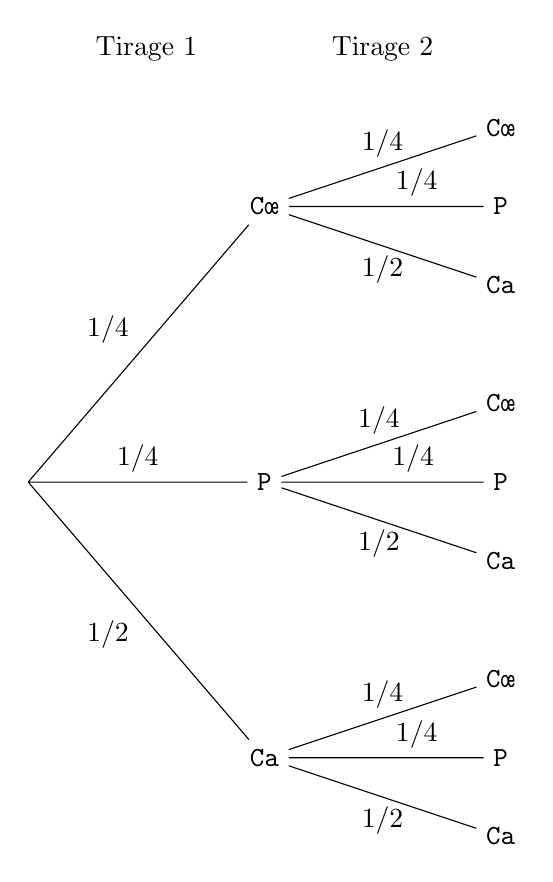
\begin{tikzpicture}
				            \coordinate (A) at (0,0);
				            \node (B1) at (3,3.5) {\correctionDots{\texttt{Cœ}}};
				            \node (B2) at (3,0) {\correctionDots{\texttt{P }}};
				            \node (B3) at (3,-3.5) {\correctionDots{\texttt{Ca}}};
				            \node (C11) at (6,4.5) {\correctionDots{\texttt{Cœ}}};
				            \node (C12) at (6,3.5) {\correctionDots{\texttt{P }}};
				            \node (C13) at (6,2.5) {\correctionDots{\texttt{Ca}}};
				            \node (C21) at (6,1) {\correctionDots{\texttt{Cœ}}};
				            \node (C22) at (6,0) {\correctionDots{\texttt{P }}};
				            \node (C23) at (6,-1) {\correctionDots{\texttt{Ca}}};
				            \node (C31) at (6,-2.5) {\correctionDots{\texttt{Cœ}}};
				            \node (C32) at (6,-3.5) {\correctionDots{\texttt{P }}};
				            \node (C33) at (6,-4.5) {\correctionDots{\texttt{Ca}}};
				            \draw (A) -- node[above left] {\correction{$1/4$}} (B1)
				            (A) -- node[above] {\correction{$1/4$}} (B2)
				            (A) -- node[below left] {\correction{$1/2$}} (B3);
				            \draw (B1) -- node[above] {\correction{$1/4$}} (C11)
				            (B1) -- node[above right] {\correction{$1/4$}} (C12)
				            (B1) -- node[below] {\correction{$1/2$}} (C13);
				            \draw (B2) -- node[above] {\correction{$1/4$}} (C21)
				            (B2) -- node[above right] {\correction{$1/4$}} (C22)
				            (B2) -- node[below] {\correction{$1/2$}} (C23);
				            \draw (B3) -- node[above] {\correction{$1/4$}} (C31)
				            (B3) -- node[above right] {\correction{$1/4$}} (C32)
				            (B3) -- node[below] {\correction{$1/2$}} (C33);

										\node at (1.5,5.5) {Tirage 1};
										\node at (4.5,5.5) {Tirage 2};
			            \end{tikzpicture}
		            \end{center}
		      \item Quelle est alors la probabilité que la première carte soit un cœur, et la deuxième un trèfle ou un carreau ? \correctionDots{$1/8$}
		      \item Quelle est la probabilité de tirer exactement une carte de cœur ? \correctionOr{{\color{red}$1/16 + 1/8 + 1/16 + 1/8 = 3/8$}}{............}
		      \item On dit qu'il y a \textbf{équiprobabilité} si toutes les issues ont la même probabilité.

		            Y a-t-il équiprobabilité dans la situation de la question $2$ ? Justifier. \correctionOr{{\color{red}Non, car $1/4$ et $1/2$.}}{................................}
	      \end{enumerate}

	\item Toujours dans la situation où on tire deux cartes, on considère maintenant les évènements suivants :
	      \begin{itemize}
		      \item $A$: «La \textit{première} carte est un cœur»
		      \item $B$: «La \textit{deuxième} carte est inférieure ou égale à $3$»
	      \end{itemize}
	      \begin{enumerate}
		      \item Représenter la situation par un arbre de probabilités.
		      \item Quel évènement à la plus haute probabilité :
		            \begin{itemize}
			            \item La première carte est un cœur, la deuxième est strictement supérieure à $3$.
			            \item La première carte n'est pas un cœur, la deuxième est inférieure ou égale à $3$.
		            \end{itemize}
		            ?
	      \end{enumerate}
\end{enumerate}

\end{document}